%%%%%%%%%%%%%%%%%%%% author.tex %%%%%%%%%%%%%%%%%%%%%%%%%%%%%%%%%%%
%
% sample root file for your "contribution" to a proceedings volume
%
% Use this file as a template for your own input.
%
%%%%%%%%%%%%%%%% Springer %%%%%%%%%%%%%%%%%%%%%%%%%%%%%%%%%%

\documentclass{./styles/svproc}
%
% RECOMMENDED %%%%%%%%%%%%%%%%%%%%%%%%%%%%%%%%%%%%%%%%%%%%%%%%%%%
%

% to typeset URLs, URIs, and DOIs
\usepackage{url}
\usepackage{cite}
\usepackage{amsmath,amssymb,amsfonts}
\usepackage{algorithmic}
\usepackage{graphicx}
\usepackage{textcomp}
\usepackage{xcolor}
\usepackage{ragged2e}
\usepackage{setspace}
\usepackage{lipsum}
\usepackage{siunitx}
\usepackage{graphicx}%
\usepackage{multirow}%
\usepackage{amsmath,amssymb,amsfonts}%
\usepackage{amsthm}%
\usepackage{mathrsfs}%
\usepackage[title]{appendix}%
\usepackage{xcolor}%
\usepackage{textcomp}%
\usepackage{manyfoot}%
\usepackage{booktabs}%
\usepackage{algorithm}%
\usepackage{algorithmicx}%
\usepackage{algpseudocode}%
\usepackage{listings}%
\usepackage{wrapfig}
\def\UrlFont{\rmfamily}

\begin{document}
\mainmatter              % start of a contribution
%
\title{VCII Based Floating Inductor}
%
\titlerunning{VCII based Floating Inductor}  % abbreviated title (for running head)
%                                     also used for the TOC unless
%                                     \toctitle is used
%
\author{Dr. Shweta Gautam \and Dr. Urvashi Bansal \and Pranav Verma \and Yash Gupta \and
Divyansh Tanwar\and Mukul Gupta }
%
\authorrunning{..} % abbreviated author list (for running head)
%
%%%% list of authors for the TOC (use if author list has to be modified)
\tocauthor{Ivar Ekeland, Roger Temam, Jeffrey Dean, David Grove,
Craig Chambers, Kim B. Bruce, and Elisa Bertino}
%
\institute{Netaji Subhas University of Technology, Delhi,\\
\email{pranavverma0510@gmail.com, divyansh.tanwar.ug20@nsut.ac.in, yg18052003@gmail.com, mukulgupta.ug20@nsut.ac.in}\\
WWW home page: \texttt{http://users/\homedir iekeland/web/welcome.html}
\and
}
\maketitle              % typeset the title of the contribution
\begin{abstract}
This paper introduces a novel implementation of a floating inductor achieved through the utilization of a second-generation voltage conveyor (VCII).This paper also focuses on designing various topologies related to flaoting inductor . A floating inductor is one that operates independently of a common ground or reference point. The circuit design is based on transistor-level configurations with 0.18 µm TSMC CMOS parameters and a ±0.9 V supply voltage. The effectiveness of the proposed circuit is validated through Spice simulations. \dots
% We would like to encourage you to list your keywords within
% the abstract section using the \keywords{...} command.
\keywords{Second Generation Voltage Conveyor II, Floating Inductor}
\end{abstract}
%
\section{Introduction}
%
Simulated inductors have surfaced as a compelling alternative to physical inductors in electronic circuit design, primarily due to the inherent limitations of their physical counterparts. Physical inductors, typically characterized by bulky size and weight, exhibit limited design flexibility and are susceptible to variations in their inductance values due to environmental factors. In contrast, simulated inductors, constructed from compact circuit elements like capacitors and operational amplifiers, offer advantages such as reduced size, enhanced flexibility, and minimal sensitivity to external influences. These attributes make simulated inductors an appealing choice for circuit designers, underscoring their significance as a research topic in contemporary electronic systems.

Voltage Conveyor-2 (VCII) is a prominent building block in analog circuit design, known for its versatility and efficiency in handling both voltage and current signals$^1$. It offers several advantages, 
such as high input and output impedance, compatibility with CMOS technology, and the ability to process various signal types. 
VCII's intrinsic flexibility and suitability for analog applications make it an attractive choice for various circuit implementations.

One specific application area of interest is the realization of floating inductors. Floating inductors, which are not referenced to a common ground, have gained significance in contemporary circuit design. Various methods exist for implementing floating inductors, including the use of gyrators, active inductors, and simulated inductors. However, the utilization of VCII as a platform for realizing floating inductors presents several notable advantages.

VCII-based floating inductors offer simpler realizations, reduced error, minimized parasitics, and lower power consumption. These attributes make VCII an appealing choice for constructing floating inductors. The flexibility of VCII allows for precise control of inductance values while maintaining compatibility with integrated circuit environments [1,2,3]. This research explores the efficacy of VCII-based floating inductors and underscores their superiority in terms of size, flexibility, and performance when compared to other methods for floating inductor implementation, ultimately demonstrating the distinct advantages of VCII in this context.


\begin{figure}[h]
\begin{center}
    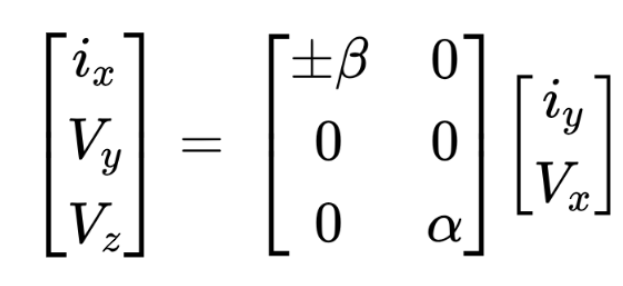
\includegraphics[width=0.3\textwidth]{templates/vc2matrix.png}
    \caption{VCII Matrix}
    \vspace{0.5cm}
  \end{center}
\end{figure}

 This component is characterized as a three-port device, designated by the labels X, Y, and Z. A notable 
distinction from CCII is that in VCII, the Y and Z terminals exhibit low impedance 
characteristics, ideally approaching zero, while the X terminal displays high impedance, 
ideally reaching infinity [1]. 
 
The outputs from each of these three ports, when considered within the context of their 
respective inputs at lower frequencies, can be expressed as shown in equation (1). 
Clearly, a VCII consists of a voltage buffer between the X and Z terminals and a current 
buffer positioned across the Y and X terminals.

The  VCII used in this work are pre-existing. Their terminal equations and voltage -current relationships have been verified using 180 nm CMOS parameters and spice tools. It is noted that following expressions are valid for the VCII$^+$ and VCII$^-$ used here:
%
\section{The Proposed VCII based designs}
The proposed VCII-based floating inductor, illustrated in Figure 3, is a noteworthy advancement in analog circuit design. Comprising two $VCII^+$ and two $VCII^-$ components, along with four strategically positioned resistors and a grounded capacitor, this implementation showcases its operational behavior through the matrix Equation (1), shedding light on its functional characteristics.
 In the context of $VCII^+$ and $VCII^-$, the current conveying operation between terminals Y and X is described by the factor + $\alpha$ for $VCII^+$ and the opposite factor for $VCII^-$. This means that $VCII^+$ and $VCII^-$ have different current gains due to the difference in the direction of current flow.
\begin{figure}[h]
\begin{center}
    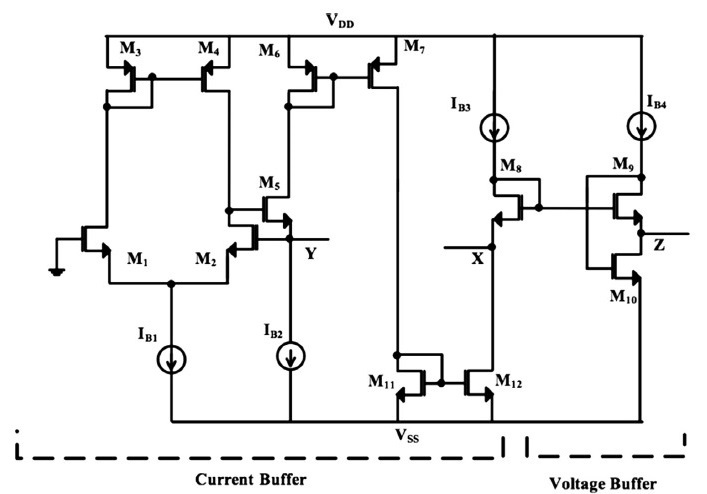
\includegraphics[width=0.6\textwidth]{CC2(2).jpg}
    \caption{$VCII^-$ Circuit Implementation [14]}
    \vspace{0.5cm}
    \includegraphics[width=0.6\textwidth]{CC2(1).jpg}
    \caption{$VCII^+$ Circuit Implementation [1]}
  \end{center}
\end{figure}

\begin{table}[h]
\centering
\caption{Transistor Dimensions for VC2 [1]}
\begin{tabular}{|c|c|c|}
\hline
Transistor & Width (µm) & Length (µm) \\
\hline
M1,M2 & 4.2 & 0.35 \\
M3,M4 & 21 & 0.35 \\
M5 & 7 & 0.35 \\
M6,M7 & 72.8 & 4.6 \\
M8,M9 & 28.7 & 1.4 \\
M10 & 14 & 52 \\
M11,M12 & 7 & 0.35 \\
\hline
\end{tabular}
\end{table}
\vspace{0.5cm}

\begin{equation}\label{assumption_matrix}
% \begin{math}
\hspace{0cm}
\begin{bmatrix}
i_1\\
i_2 
\end{bmatrix} =\frac{1}{Z} \begin{bmatrix}
1&-1\\
-1&1
\end{bmatrix} \begin{bmatrix}
v_1\\
v_2 
\end{bmatrix}   
\end{equation}
% \end{math}
\vspace{0.25cm}

\subsection{Floating Inductor}
\begin{figure}[h]
\begin{center}
    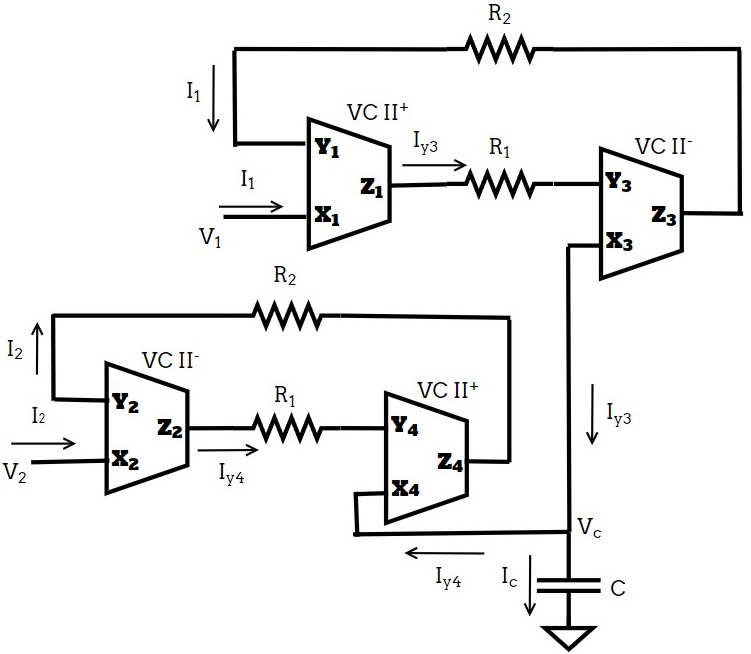
\includegraphics[width=0.7\textwidth]{floating inductor.jpg}
    \caption{Proposed Floating Inductor}
  \end{center}
\end{figure}
% \begin{figure}
% \begin{center}
%     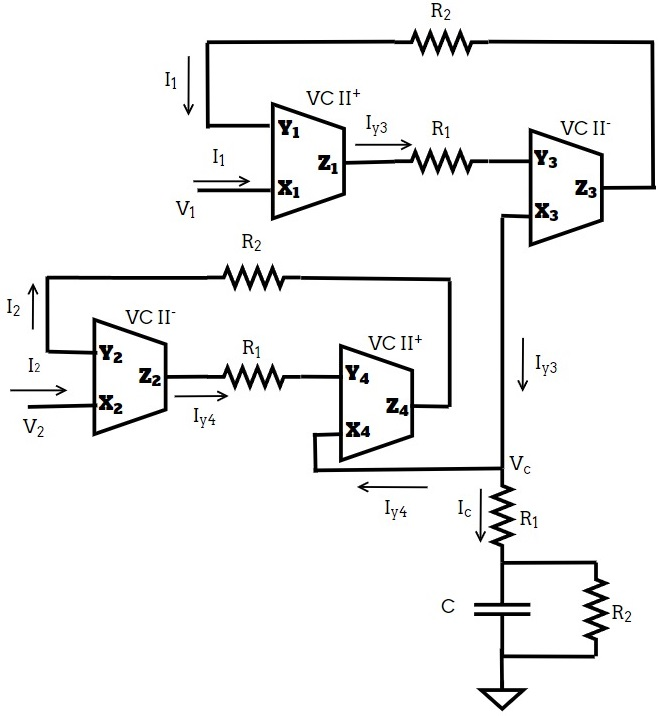
\includegraphics[width=0.40\textwidth]{advanced.jpg}
%     \caption{figure 6}
%   \end{center}
% \end{figure}

% Using \eqref{assumption_matrix} for V_{z2} and V_{z1} we have:\\

{To derive mathematical expression of a floating inductor, equation \eqref{assumption_matrix} is used for {$V_{z1},V_{z2},V_{z3},V_{z4}$}:} 

\begin{equation}\label{eq:1.0.1}
\begin{array}{l}
V_{z1}=V_1 \, , \\
V_{z2}=V_2 \,,\\
V_{z3}=V_{x3}=V_c \, ,\\ 
V_{z4}=V_{x4}=V_c
\end{array}
\end{equation}

using \eqref{assumption_matrix} for terminal currents:
\begin{equation}\label{eq:1.0.2}
\begin{array}{l}
i_{y1}=i_{x1}=I_1 \, ,\\
i_{y2}=-i_{x2}=-I_2 \,,\\
i_{x3}=-i_{y3} \, ,\\ 
i_{x4}=i_{y4}
\end{array}
\end{equation}
\begin{equation}\label{eq:1.1}
i_{y3}=\frac{V_{z1}}{R_1}=\frac{V_1}{R_1}
\end{equation}

\begin{equation}\label{eq:1.2}
i_{y4}=\frac{V_{z2}}{R_1}=\frac{V_2}{R_1}
\end{equation}

\begin{equation}\label{eq:1.3}
I_c=i_{y3}-i_{y4}
\end{equation}

using equation \eqref{eq:1.1}, \eqref{eq:1.2} and \eqref{eq:1.3}

\begin{equation}\label{eq:1.4}
I_c = \frac{V_1}{R_1} - \frac{V_2}{R_1}\\
\end{equation}

\begin{equation}\label{eq:1.5}
I_1=\frac{V_c - 0}{R_2}\\
\end{equation}

\begin{equation}\label{eq:1.8}
I_2=\frac{0-V_c}{R_2}\\
\end{equation}

\begin{equation}\label{eq:1.6}
V_c= \frac{I_c}{sC}\\
\end{equation}

using equation \eqref{eq:1.4}, \eqref{eq:1.5} and \eqref{eq:1.6}

\begin{equation}\label{eq:1.7}
I_1=\frac{V_1 - V_2}{sCR_1R_2}\\
\end{equation}

using equation \eqref{eq:1.4}, \eqref{eq:1.8} and \eqref{eq:1.6}

\begin{equation}\label{eq:1.9}
I_2=\frac{V_2-V_1}{s CR_1R_2}\\
\end{equation}

\begin{equation}\label{eq:1.10}
\frac{V_2-V_1}{I_2}=s CR_1R_2\\
\end{equation}

\subsection{Series Inductor with resistance}
The equation \eqref{eq:1.0.1}-\eqref{eq:1.8} remain same for all implementation in this paper

\begin{figure}[h]
\begin{center}
    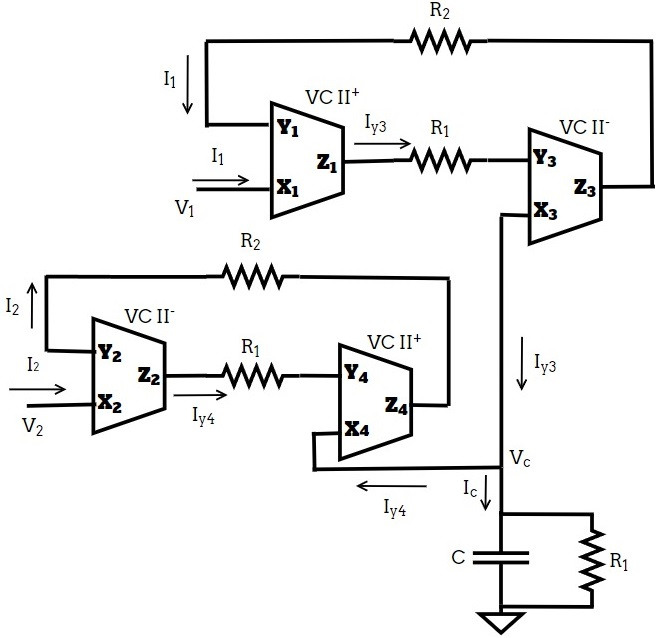
\includegraphics[width=0.6\textwidth]{series.jpg}
    \caption{Floating Series RL Impedance}
  \end{center}
\end{figure}

% --\\-----------\\
% for z= sL parallel R\\
% (figure 4)\\
% -------\\

\begin{equation}\label{eq:2.1}
V_c=I_c \left( \frac{1}{sC}+R \right)
\end{equation}

using \eqref{eq:1.4}, \eqref{eq:1.5} and \eqref{eq:2.1}

\begin{equation}\label{eq:2.2}
I_1=\frac{V_1-V_2}{R_1R_2} \left( \frac{1}{sC}+R \right)
\end{equation}

\begin{equation}\label{eq:2.3}
Z_{in}=\frac{V_1-V_2}{I_1} = \frac{sCR_1R_2}{sCR_1+1}
\end{equation}

\begin{equation}\label{eq:2.4}
\frac{1}{Z_{in}} = \frac{1}{sCR_1R_2}+\frac{1}{R_2}
\end{equation}



\begin{figure}[h]
\begin{center}
     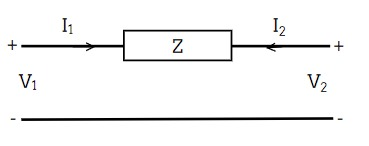
\includegraphics[width=0.45\textwidth]{templates/Generalfig.jpg}
    \caption{General Equivalent Floating Inductor}
  \end{center}
\end{figure}

\begin{equation}\label{eq:2.4}
{Z} = {R}+{sL_eq}
\end{equation}



\subsection{Parallel Inductor with resistance}
% --\\-----------\\
% for z= sL + R\\
% (figure 6)\\
% -------\\
\begin{figure}[h]
\begin{center}
    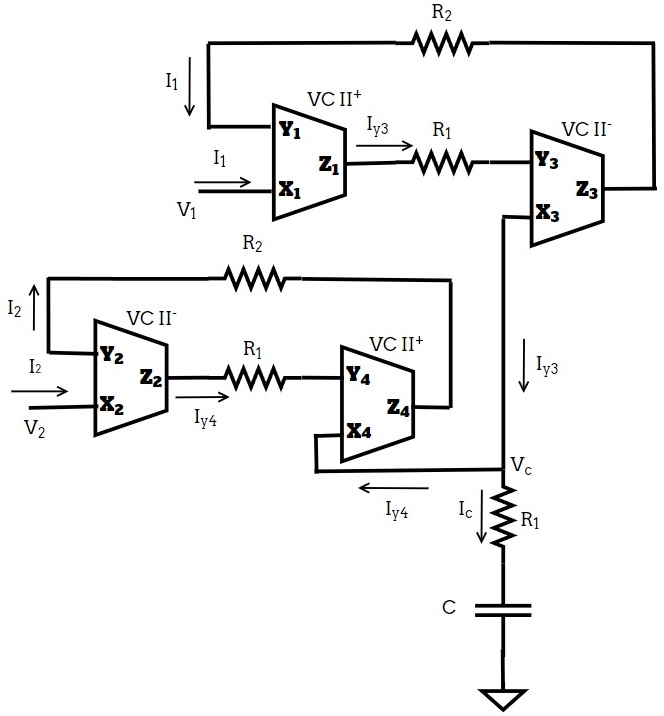
\includegraphics[width=0.47\textwidth]{parallel.jpg}
    \caption{Floating Parallel RL Impedance}
  \end{center}
\end{figure}



\begin{equation}\label{eq:3.1}
V_c=I_c \left( \frac{R_1}{sCR_1 +1} \right)
\end{equation}

using \eqref{eq:1.4}, \eqref{eq:1.5} and \eqref{eq:3.1}

\begin{equation}\label{eq:3.2}
I_1=\frac{V_1-V_2}{R_1R_2} \left( \frac{R_1}{sCR_1 +1} \right)
\end{equation}

\begin{equation}\label{eq:3.3}
Z_{in}=\frac{V_1-V_2}{I_1} = sCR_1R_2 + R_2
\end{equation}
Equivalent floating inductor with resistance in parallel can be observed from figure 5 where

\begin{equation}\label{eq:3.4}
{Z} = {R}\parallel{sL}
\end{equation}

% \begin{figure}[h]
% \begin{center}
%      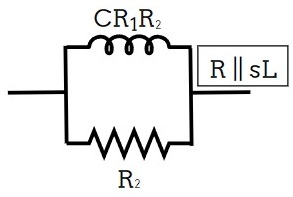
\includegraphics[width=0.3\textwidth,width=0.35\columnwidth]{pareq.jpg}
%     \caption{Equivalent Floating Inductor with resistance in parallel}
%   \end{center}
% \end{figure}



\subsection{Mixed implementaion of series and parallel resistance with inductor}
% --\\-----------\\
% for z= sL + R parallel R\\
% (figure 8)\\
% -------\\
\begin{figure}[h]
\begin{center}
    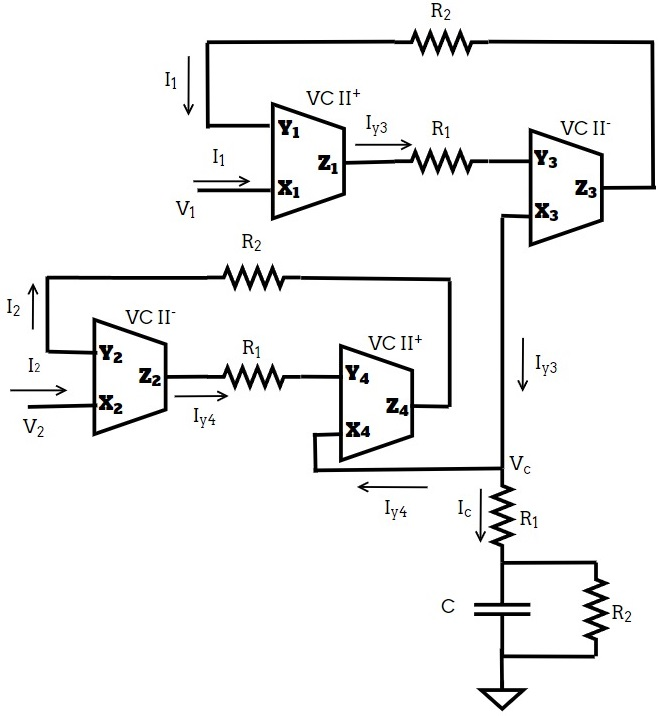
\includegraphics[width=0.4\textwidth]{advanced.jpg}
    \caption{Floating Series Parallel RL Impedance}
  \end{center}
\end{figure}

\begin{equation}\label{eq:4.1}
V_c=I_c \left( \frac{sCR_1R_2+R_1+R_2}{sCR_2 +1} \right)
\end{equation}

using \eqref{eq:1.4}, \eqref{eq:1.5} and \eqref{eq:4.1}

\begin{equation}\label{eq:4.2}
I_1=\frac{V_1-V_2}{R_1R_2} \left( \frac{sCR_1R_2+R_1+R_2}{sCR_2 +1} \right)
\end{equation}

\begin{equation}\label{eq:4.3}
Z_{in}=\frac{V_1-V_2}{I_1} = \frac{R_2(sCR_1R_2+R1)}{R_2+(sCR_1R_2+R1)}
\end{equation}

\begin{equation}\label{eq:4.4}
\frac{1}{Z_{in}}= \frac{1}{R_2}+\frac{1}{sCR_1R_2+R1}
\end{equation}

% \begin{figure}[h]
% \begin{center}
%      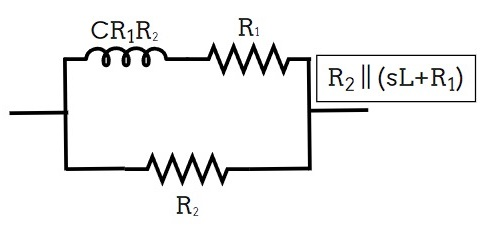
\includegraphics[width=0.5\textwidth]{adveq.jpg}
%     \caption{Equivalent Floating Inductor with resistance in parallel and series}
%   \end{center}
% \end{figure}
Equivalent floating inductor with resistance in parallel and series can be observed from figure 5 where

\begin{equation}\label{eq:3.4}
{Z} = {R_2}\parallel{(sL+R_1)}
\end{equation}

\section{Applications}
The functionality of our VCII was evaluated using a variety of applications. A standard RLC bandpass filter was successfully implemented, demonstrating the versatility of the VCII. We also conducted tests to evaluate the resilience and durability of the design.

\subsection{RLC Bandpass Filter}\label{AA}
\begin{figure}[h]
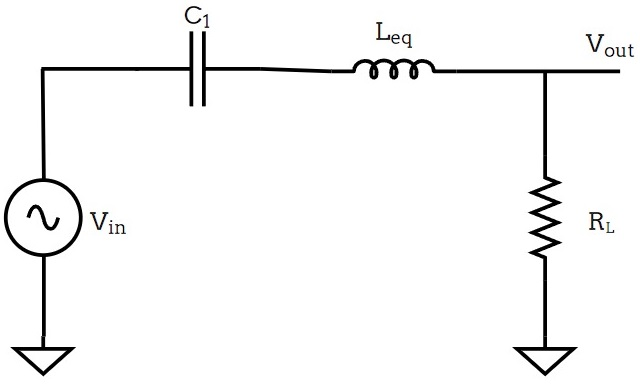
\includegraphics[width=0.55\textwidth]{application1.jpg}
\centering
\caption{RLC Bandpass filter}
\end{figure}
An RLC band-pass filter is a type of filter that allows frequencies within a specific range and rejects frequencies outside that range. It’s made up of a resistor $R_L$ = 10k$\si{\ohm}$, our proposed floating inductor ($L_{eq}$), and capacitor $C_1$ = 50pf.

The band-pass filter is a combination of low pass and high pass filters. The low pass filter isolates the signals which have frequencies higher than the cutoff frequency, and the high pass filter isolates the signals which have frequencies lower than the cutoff frequency.

\section{Simulations \& Results}

Simulation using LTSpice was conducted on the floating inductors depicted in Figure 11, utilizing a 0.18 $\mu$m CMOS technology and a supply voltage of ±0.9 V. The aspect ratios for the PMOS and NMOS transistors used are detailed in Table 1. The bias currents were set at $I_{B1}$ = 30 $\mu$A, $I_{B2}$ = $I_{B3}$ = $I_{B4}$ = 20 $\mu$A, all implemented through simple current mirrors.

\begin{figure}[h]
\begin{center}
    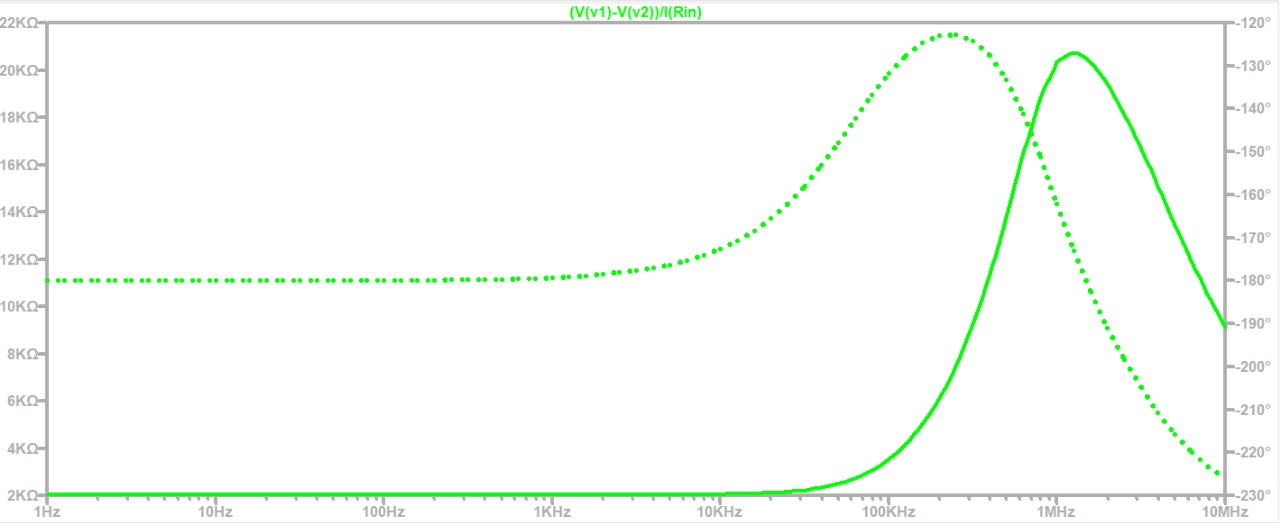
\includegraphics[width=1\textwidth]{WhatsApp Image 2023-11-20 at 15.28.38_cffe913f.jpg}
    \caption{Floating Inductor - I}
 \end{center}
\end{figure}


\begin{figure}[h]
\begin{center}    
    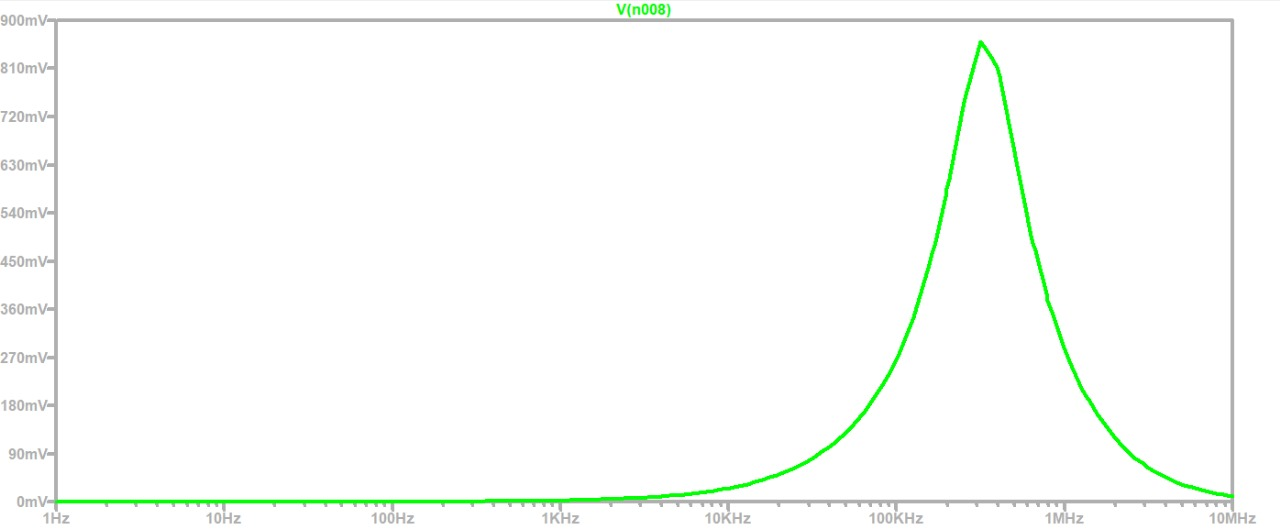
\includegraphics[width=1\textwidth]{rlc app sim2.jpg}
    \caption{Floating Inductor - II}
  \end{center}
\end{figure}


For a capacitance value of $C_{1}$ = 50 pF, Figure x displays the magnitude and phase frequency response of the proposed floating inductor within the frequency range of 200 kHz to 1 MHz.

The performance assessment of the proposed floating inductor was carried out within a standard RLC band-pass filter configuration, with $C_{1}$ = 50 pF and $R_{L}$ = 10 k$\si{\ohm}$ as shown in Figure x. The simulated resonant frequency ($f_{0}$) was determined to be 318.67 kHz, as illustrated in Figure x showcasing the frequency response of the RLC band-pass filter utilizing the simulated inductance.


The topology described in [10] incorporates a floating capacitor, introducing a notable disadvantage. The use of a floating capacitor in this configuration hinders integration, making the overall design less favorable from that perspective.

In [15], a distinct topology is employed, featuring CCII±, a dual output transconductance amplifier (DO-OTA), one resistor, and one floating capacitor. However, a noteworthy drawback is associated with the use of a floating capacitor.

This novel active building block, referred to as a second-generation voltage conveyor (VCII) [19,6,20,19,20], serves as the dual counterpart to the well-established CCII. It has been integrated into the construction of grounded impedance simulators [21,3]. A comparison highlights that the simulated grounded capacitors and inductors utilizing VCII offer numerous advantages, including simpler realizations, reduced errors, minimized parasitics, lower power consumption, and more, in contrast to simulated grounded impedances employed by other active building blocks (ABBs). The reported findings in [21,22] suggest that the incorporation of VCII in impedance simulators holds considerable promise.

\section{Conclusion}
This research paper introduces a novel implementation of a floating inductor using a second-generation voltage conveyor (VCII). It discusses limitations of physical inductors, highlights advantages of simulated inductors, and emphasizes the versatility of VCII in handling both voltage and current signals. This paper introduces a novel topology for realizing a floating inductor multiplier, utilizing two VCII+ and two VCII−, along with a single grounded capacitor and some resistors,  implemented using a 180 nm cmos technology. Various configurations of floating inductors are presented, demonstrating series, parallel, and mixed topologies, with accompanying mathematical derivations. The practical application of the proposed circuit as a standard RLC filter is also provided to validate its functionality.


% \section*{Acknowledgment}

% We would like to express my gratitude and appreciation to all those who make it possible to complete this paper. Special thanks to our project supervisor(s) Dr. Shweta Gautam and Dr. Urvashi Bansal whose help, stimulating suggestions and encouragement helped us in writing this report. We also sincerely thank our colleagues for the time spent proofreading and correcting our mistakes. 

\begin{thebibliography}{00}
\bibitem{b1} L. Safari et al., "High performance voltage output filter realizations using second generation voltage conveyor," *Int. J. RF Microw. Comput. Aided Eng.*, vol. 28, no. 6, pp. 1-5, 2018. DOI: 10.1002/mmce.21534.

\bibitem{b2}V. Stornelli, L. Safari, G. Barile, and G. Ferri, "A new VCII based grounded positive/negative capacitance multiplier," *AEU - International Journal of Electronics and Communications*, vol. 137, p. 153793, 2021.

\bibitem{b3} Smith, J., \& Jones, K. (2020). A second‐generation voltage conveyor (VCII)–based simulated grounded inductor. International Journal of Circuit Theory and Applications, 48(11), 1234-1245.

\bibitem{b4} R. Senani, "New Tunable Synthetic Floating Inductors," Electronics Letters, vol. 16, no. 10, p. 382, 1980.

\bibitem{b5} J. Cajka and K. Vrba, "The Voltage Conveyor May Have in Fact Found its Way into Circuit Theory," *Int. J. Electron. Commun. (AEU)*, vol. 58, pp. 244-248, 2004. [Online].

\bibitem{b6} L. Safari et al., "An overview on the second generation voltage conveyor: Feature, design and applications," *IEEE Trans. Circuits Syst. II Express Briefs*, vol. 66, no. 4, pp. 547-551, Apr. 2019.

\bibitem{b7} F. Centurelli et al., "On the use of voltage conveyors for the synthesis of biquad filters and arbitrary networks," in *2017 European Conference on Circuit Theory and Design (ECCTD)*, Catania, Italy, 2017, pp. 1-4.

\bibitem{b8} H. Uhrmann et al., "Current-Mode Filters," in *Analog Filters in Nanometer CMOS*, Springer Series in Advanced Microelectronics, vol. 45, Berlin, Heidelberg: Springer, 2014.

\bibitem{b9} C.K. Smith and A. Sedra, "The current conveyor – a new building block," in *IEEE Proc.*, vol. 56, pp. 1368-1369, 1968.

\bibitem{b10} A. Sedra and C.K. Smith, "A second-generation current conveyor and its applications," in *IEEE Trans. on Circuit Theory*, vol. CT-17, pp. 132-134, 1970.
\bibitem{b11} H. Uhrmann, R. Kolm, H. Zimmermann, "Current-Mode Filters," *Analog Filters in Nanometer CMOS*, Springer Series in Advanced Microelectronics, vol. 45, Berlin, Heidelberg: Springer, 2014.

\bibitem{b12} L. Safari, G. Barile, V. Stornelli, and G. Ferri, "An Overview on the Second Generation Voltage Conveyor: Features, Design and Applications," IEEE Transactions on Circuits and Systems—II: Express Briefs, vol. 66, no. 4, pp. 547–551, April 2019.

\bibitem{b13} P. Ahmadi, M. Taghavi, L. Belostotski, "A 0.13-µm CMOS current-mode all-pass filter for multi-GHz operation," *IEEE Trans. Very Large Scale Integr(VLSI) Syst.*, vol. 23, no. 12, pp. 2813-2818, 2015.

\bibitem{b14} M. A. Al-Absi, "Realization of inverse filters using second-generation voltage conveyor (VCII)," *Analog Integrated Circuits and Signal Processing*, vol. 109, pp. 29-32, May 2021. DOI: 10.1007/s10470-021-01874-3.

\bibitem{b15} G. Barile, L. Safari, G. Ferri, and V. Stornelli, "Traditional Op-Amp and New VCII: A Comparison on Analog Circuits Applications," AEU - International Journal of Electronics and Communications, p. 152845, 2019.

\bibitem{b16} A. Khan and M. H. Zaidi, "A Novel Ideal Floating Inductor Using Translinear Conveyors," Active and Passive Electronic Components, vol. 26, no. 2, pp. 87–89, 2003.

\bibitem{b17} R. G. Carvajal et al., "The Flipped Voltage Follower: A Useful Cell for Low-Voltage Low-Power Circuit Design," *IEEE Trans. Circuits Syst. I Regul. Pap.*, vol. 52, no. 7, pp. 1317-1326, Jul. 2005.

\bibitem{b18}L. Safari and S. J. Azhari, "A New Low Voltage Low Power Fully Differential Current Buffer and Its Application as a Voltage Amplifier," *Int. J. Model. Optim.*, vol. 2, no. 3, pp. 274-278, Jun. 2012.

\bibitem{b19}Čajka, J.; Vrba, K. The Voltage Conveyor May Have in Fact Found its Way into Circuit Theory. AEU Int. J. Electron. Commun. 2004, 58, 244–248.


\bibitem{b20}Safari, L.; Barile, G.; Stornelli, V.; Ferri, G.; Leoni, A. New Current Mode Wheatstone Bridge Topologies with Intrinsic Linearity. In Proceedings of the 14th Conference on Ph.D. Research in Microelectronics and Electronics (PRIME), Prague, Czech Republic, 2–5 July 2018; IEEE: Piscataway, NJ, USA, 2018; pp. 9–12.

\bibitem{b21}Stornelli, V.; Safari, L.; Barile, G.; Ferri, G. A New Extremely Low Power Temperature Insensitive Electronically Tunable VCII-Based Grounded Capacitance Multiplier. IEEE Trans. Circuits Syst. II Express Briefs 2021, 68, 72–76.


\end{thebibliography}
\vspace{12pt}

%
% ---- Bibliography ----
%

\end{document}
